\section{Auswertung}
\label{sec:Auswertung}
\subsection{Verwertung der Messwerte zur zeitabhängigkeit der Amplitude}
\label{subsec:AuswertungA}

Um den effektiven Dämpfungswiderstand zu bestimmen kann man folgende Formel betrachten: 
\begin{equation}
  \label{eqn:Abklingdauer}
  \frac{1}{2\pi\mu} = \frac{2L}{R_{\text{eff}}}
\end{equation}
Durch Umstellen auf $R_{\text{eff}}$ ergibt sich eine Berechnungsformel:
\begin{equation}
  \label{Abklingdauer1}
  \Longleftrightarrow R_{\text{eff}} = 4\pi\mu L
\end{equation}
Um nun $R_{\text{eff}}$ zu berechnen wird zunächst eine Fit-Kurve durch die Messwerte gelegt (siehe \autoref{fig:PlotZuA}).

\-\begin{figure}
  \centering
  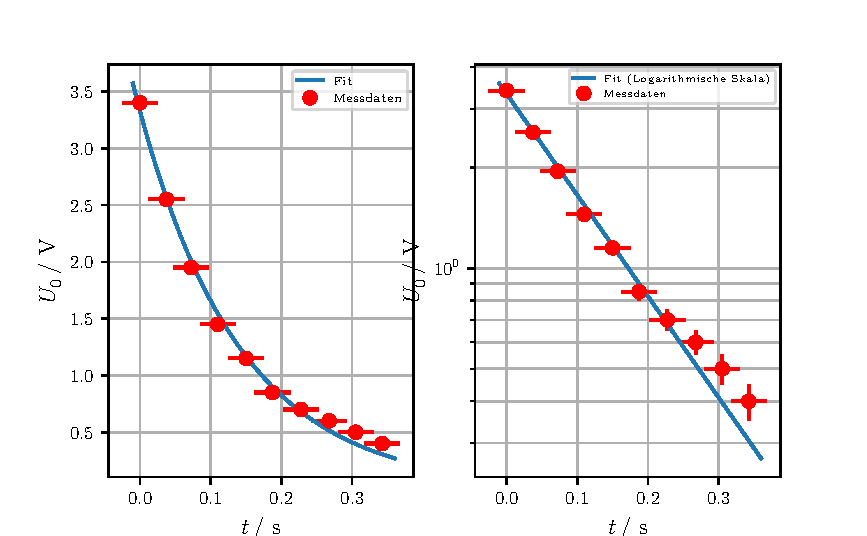
\includegraphics[width=0.7\textwidth]{PlotZuA.pdf}
  \caption{Exponentieller Fit zu den Messwerten mit linearer Skala (links) und logarithmischer Skala für $U$ (rechts)}
  \label{fig:PlotZuA}
\end{figure}

Man benötigt nun noch den Faktor $2\pi\mu$. Diesen kann man durch die erstellte exponentielle Regression 
bestimmen, da $2\pi\mu$ dem positiven Faktor des Exponenten der erstellten Exponentialfunktion entspricht. 
Daher ist $2\pi\mu = 6.98\unit{\second}$.
$R_{\text{eff}}$ ergibt sich durch einsetzen zu:
\begin{equation*}
  R_{\text{eff}} = (2\cdot 6.98\cdot \num{16.87\pm 0.05}) \unit{\ohm} = (\num{117.75 \pm 0.05})\,\unit{\ohm}
\end{equation*}

\subsection{Aperiodischer Grenzfall}
\label{subsec:AuswertungB}

Der Theoriewert des Widerstands, bei dem der aperiodische Grenzfall eintritt, lässt sich mit Formel \eqref{eqn:R_ap} berechnen.
Der Fehler dieses Wertes ergibt sich nach der gaußschen Fehlerfortpflanzung zu:

\begin{align*}
  \label{eqn:err_R_ap}
  \Delta R_{\text{ap}} &= \sqrt{\Bigl(\frac{\symup{d}R_{\text{ap}}}{\symup{d}L}\Delta L \Bigr)^2+\Bigl(\frac{\symup{d}R_{\text{ap}}}{\symup{d}C}\Delta C\Bigr)^2} \\
  &= \sqrt{\Bigl(\frac{1}{\sqrt{LC}}\Delta L\Bigr)^2+\Bigl(\frac{\sqrt{LC}}{C^2}\Delta C\Bigr)} \\
  &\approx 43 \unit{\ohm}
\end{align*}

Insgesamt erhält man $R_{\text{ap, Theorie}} = (5,72 \pm 0,043) \unit{\kilo\ohm}$. Der experimentell ermittelte Wert wurde 
zu $R_{\text{ap, exp}} = (4,49 \pm 0,01) \unit{\kilo\ohm}$ bestimmt.

\subsection{frequenzabhängigkeit der Kondensatorspannung}
\label{subsec:AuswertungC}

